\documentclass[tikz]{standalone}
\usetikzlibrary{positioning}
% newcommands.tex

\newcommand{\enq}{\texttt{enq}}
\newcommand{\deq}{\texttt{deq}}
\newcommand{\pput}{\texttt{PUT}}
\newcommand{\get}{\texttt{GET}}
\newcommand{\vs}{\texttt{vis}}
\newcommand{\so}{\texttt{so}}
\newcommand{\arb}{\texttt{ar}}
\newcommand{\rf}{\texttt{rf}}

% example
\newcommand{\po}[2]{\draw [->, thick] (#1) to node[above] {\Large{\so}} (#2);}
\newcommand{\pva}[2]{\draw [->, thick] (#1) to node[above] {$\Large{\so},\Large{\vs},\Large{\arb}$} (#2);}
\newcommand{\pbva}[2]{\draw [->, thick] (#1) to node[above] {$\Large{\so}$} node[below] {$\Large{\vs},\Large{\arb}$} (#2);}
\newcommand{\pv}[2]{\draw [->, thick] (#1) to node[above] {\Large{\so}} node[below] {\Large{\vs}} (#2);}
\newcommand{\evis}[2]{\draw [->, thick] (#1) to node[above, sloped, near end] {\Large{\vs}} (#2);}
\newcommand{\mvis}[2]{\draw [->, thick] (#1) to node[above, sloped] {\Large{\vs}} (#2);}
\newcommand{\ar}[2]{\draw [->, thick, allow upside down] (#1) to node[above, sloped] {\Large{\arb}} (#2);}
\newcommand{\va}[2]{\draw [->, thick, allow upside down] (#1) to node[above, sloped] {$\Large{\vs},\Large{\arb}$} (#2);}
\newcommand{\vab}[2]{\draw [->, thick, allow upside down] (#1) to node[below, sloped, near end] {$\Large{\vs},\Large{\arb}$} (#2);}
\newcommand{\vae}[2]{\draw [->, thick, allow upside down] (#1) to node[above, sloped, near end] {$\Large{\vs},\Large{\arb}$} (#2);}
\newcommand{\vas}[2]{\draw [->, thick, allow upside down] (#1) to node[sloped, near start, above] {$\Large{\vs},\Large{\arb}$} (#2);}

% serialization
\newcommand{\scc}[2]{\draw [->, very thick] (#1) to (#2);}
\newcommand{\rva}[2]{\draw [->, thick, allow upside down] (#1) to node[above, sloped] {$\Large{\rf},\Large{\vs},\Large{\arb}$} (#2);}
\newcommand{\rvb}[2]{\draw [->, thick, allow upside down] (#1) to node[below, sloped] {$\Large{\rf},\Large{\vs},\Large{\arb}$} (#2);}


\begin{document}
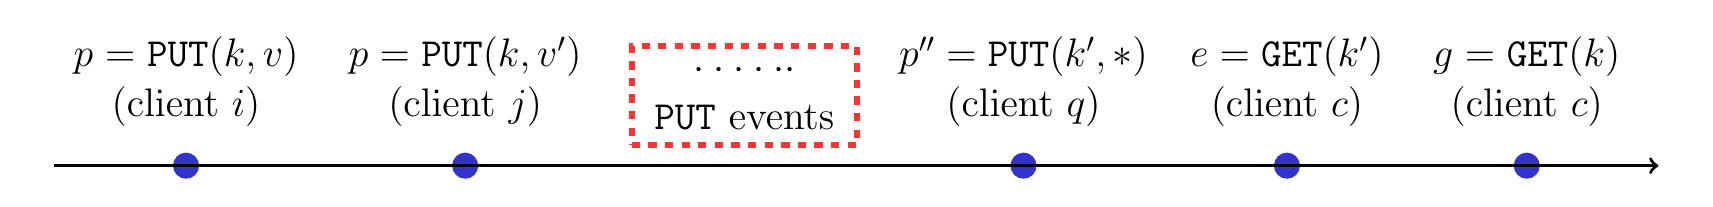
\begin{tikzpicture}
\tikzset{
 pu/.style = {rectangle, font =\Large, text width=9em, text centered},
 put/.style = {rectangle, font =\Large, text width=8.5em, text centered},
 get/.style = {rectangle, font =\Large, text width=7em, text centered}, 
 d/.style = {circle, radius = 0.3cm},
 dot/.style = {circle, radius = 2ex, fill = blue!80!yellow},
 dots/.style = {rectangle, dashed, line width = 0.5ex, font=\Large, draw = red!80!white, text width=7em, inner sep = 0.2cm, text centered},
}
  \node (start) [d] {};
  \node (c1) [dot, right = 1.5cm of start] {};
  \node (c2) [dot, right = 3.2cm of c1] {};
  \node (c3) [d, right = 3.2cm of c2] {};
  \node (c4) [dot, right = 3.2cm of c3] {};
  \node (c5) [dot, right = 3cm of c4] {};    
  \node (c6) [dot, right = 2.7cm of c5] {};   
  \node (end) [d, right = 1.5cm of c6] {};
  \scc{start}{end};

  \node (p) [put, above = 0.2cm of c1] {$p=\pput(k,v)$ \\ (client $i$)};
  \node (p') [put, above = 0.2cm of c2] {$p=\pput(k,v')$ \\ (client $j$)};
  \node (dot) [dots, above = 0.05cm of c3] {$\bf{\cdot\cdot\cdot\cdot\cdot\cdot}$ \\ \pput{} events};
  \node (p'') [pu, above = 0.2cm of c4] {$p''=\pput(k',\ast)$ \\ (client $q$)};
  \node (e) [get, above = 0.2cm of c5] {$e = \get(k')$ \\ (client $c$)};
  \node (g) [get, above = 0.2cm of c6] {$g = \get(k)$ \\ (client $c$)};

\end{tikzpicture}
\end{document}
